\documentclass[a4paper,12pt]{report} %%%{article}

\usepackage{cmap} % searchable PDFs
\usepackage[T2A]{fontenc} % scalable fonts
\usepackage[utf8]{inputenc} % input in UTF8
%\usepackage[english,russian]{babel} % dashes on linebreaks
\usepackage{indentfirst} % indents in paragraphs
\usepackage{amstext,amssymb,amsfonts,amsmath,mathtext,enumerate,float}
\usepackage[left=25mm,right=2cm,top=2cm,bottom=2cm,bindingoffset=0cm]{geometry}
\usepackage[unicode]{hyperref}
\usepackage{graphicx}
\usepackage{ulem} % strikethrough
\usepackage{verbatim} % multiline comments
\usepackage{hhline}

\usepackage{listings}
\usepackage{color}
 
\definecolor{dkgreen}{rgb}{0,0.6,0}
\definecolor{gray}{rgb}{0.5,0.5,0.5}
\definecolor{mauve}{rgb}{0.58,0,0.82}
 
\lstset{ %
  columns=flexible,
%  language=C,                     % the language of the code
  basicstyle=\footnotesize\ttfamily,       % the size of the fonts that are used for the code
  numbers=left,                   % where to put the line-numbers
  numberstyle=\tiny\color{gray},  % the style that is used for the line-numbers
  stepnumber=1,                   % the step between two line-numbers. If it's 1, each line 
                                  % will be numbered
  numbersep=5pt,                  % how far the line-numbers are from the code
  backgroundcolor=\color{white},  % choose the background color. You must add \usepackage{color}
  showspaces=false,               % show spaces adding particular underscores
  showstringspaces=false,         % underline spaces within strings
  showtabs=false,                 % show tabs within strings adding particular underscores
%  frame=single,                   % adds a frame around the code
  rulecolor=\color{black},        % if not set, the frame-color may be changed on line-breaks within not-black text (e.g. comments (green here))
  tabsize=4,                      % sets default tabsize
  captionpos=b,                   % sets the caption-position to bottom
  breaklines=true,                % sets automatic line breaking
  breakatwhitespace=false,        % sets if automatic breaks should only happen at whitespace
  title=\lstname,                 % show the filename of files included with \lstinputlisting;
                                  % also try caption instead of title
  keywordstyle=\color{blue},      % keyword style
  commentstyle=\color{dkgreen},   % comment style
  stringstyle=\color{mauve},      % string literal style
%  escapeinside={\%*}{*)},         % if you want to add LaTeX within your code
  mathescape=true,
  morekeywords={*,...},           % if you want to add more keywords to the set
  deletekeywords={...}            % if you want to delete keywords from the given language
}

\lstset{
literate={а}{{\selectfont\char224}}1
{б}{{\selectfont\char225}}1
{в}{{\selectfont\char226}}1
{г}{{\selectfont\char227}}1
{д}{{\selectfont\char228}}1
{е}{{\selectfont\char229}}1
{ё}{{\"e}}1
{ж}{{\selectfont\char230}}1
{з}{{\selectfont\char231}}1
{и}{{\selectfont\char232}}1
{й}{{\selectfont\char233}}1
{к}{{\selectfont\char234}}1
{л}{{\selectfont\char235}}1
{м}{{\selectfont\char236}}1
{н}{{\selectfont\char237}}1
{о}{{\selectfont\char238}}1
{п}{{\selectfont\char239}}1
{р}{{\selectfont\char240}}1
{с}{{\selectfont\char241}}1
{т}{{\selectfont\char242}}1
{у}{{\selectfont\char243}}1
{ф}{{\selectfont\char244}}1
{х}{{\selectfont\char245}}1
{ц}{{\selectfont\char246}}1
{ч}{{\selectfont\char247}}1
{ш}{{\selectfont\char248}}1
{щ}{{\selectfont\char249}}1
{ъ}{{\selectfont\char250}}1
{ы}{{\selectfont\char251}}1
{ь}{{\selectfont\char252}}1
{э}{{\selectfont\char253}}1
{ю}{{\selectfont\char254}}1
{я}{{\selectfont\char255}}1
{А}{{\selectfont\char192}}1
{Б}{{\selectfont\char193}}1
{В}{{\selectfont\char194}}1
{Г}{{\selectfont\char195}}1
{Д}{{\selectfont\char196}}1
{Е}{{\selectfont\char197}}1
{Ё}{{\"E}}1
{Ж}{{\selectfont\char198}}1
{З}{{\selectfont\char199}}1
{И}{{\selectfont\char200}}1
{Й}{{\selectfont\char201}}1
{К}{{\selectfont\char202}}1
{Л}{{\selectfont\char203}}1
{М}{{\selectfont\char204}}1
{Н}{{\selectfont\char205}}1
{О}{{\selectfont\char206}}1
{П}{{\selectfont\char207}}1
{Р}{{\selectfont\char208}}1
{С}{{\selectfont\char209}}1
{Т}{{\selectfont\char210}}1
{У}{{\selectfont\char211}}1
{Ф}{{\selectfont\char212}}1
{Х}{{\selectfont\char213}}1
{Ц}{{\selectfont\char214}}1
{Ч}{{\selectfont\char215}}1
{Ш}{{\selectfont\char216}}1
{Щ}{{\selectfont\char217}}1
{Ъ}{{\selectfont\char218}}1
{Ы}{{\selectfont\char219}}1
{Ь}{{\selectfont\char220}}1
{Э}{{\selectfont\char221}}1
{Ю}{{\selectfont\char222}}1
{Я}{{\selectfont\char223}}1
}
\usepackage{mathtools}
\newcommand{\defeq}{\vcentcolon=}
\newcommand{\eqdef}{=\vcentcolon}

\renewcommand{\contentsname}{Содержание} 
\setcounter{secnumdepth}{0}
\setcounter{tocdepth}{3}

%\sloppy % align=justify

% \title{Схема сборки проекта с~агрессивным переиспользованием порождений}
	   
\author[Сергей Серебряков]{Сергей Серебряков}

\institute[СПбГУ]{
	\textbf{кафедра системного программирования}\\ 
	\textbf{математико-механический ф-т, СПбГУ}\\
	\texttt{sergey@serebryakov.info}
}

\date{
	\textbf{СПИСОК-2013}
}
\title{Схема сборки проектов с~агрессивным переиспользованием порождений}
% \title[{\makebox[.45\paperwidth]{\hfill\insertframenumber/\inserttotalframenumber}}]{
% 	Схема сборки проектов с~агрессивным переиспользованием порождений
% }

\author[Сергей Серебряков]{
  \text{Сергей Серебряков, 545 группа}\\
}

\institute[]{
  \begin{tabular}[h]{rl}
      Научный руководитель: &к.ф.-м.н.~Д.~Ю.~Булычев \\
      Рецензент: &к.ф.-м.н.~Н.~В.~Чашников
  \end{tabular}      
}

\date{13 июня 2013}


\begin{document}

{
	\setbeamertemplate{footline}{}
	\begin{frame}
		\titlepage
	\end{frame}
}
\addtocounter{framenumber}{-1}

\begin{frame}{Введение}
\begin{itemize}
	\item Сборка программного проекта
	\item Инкрементальная компиляция
	\item Кэш компиляции
	\item Переиспользование кэшей в большом проекте
\end{itemize}
\begin{figure}[!h]
	\begin{center}
		\includegraphics[width=80mm]{network.png}
	\end{center}
\end{figure}
\end{frame}

\begin{frame}{Пример на Java}
\begin{figure}[!h]
	\centering
	\includegraphics[width=90mm]{state1.png}
\end{figure}
\end{frame}

\begin{frame}{Пример на Java}
\begin{figure}[!h]
	\centering
	\includegraphics[width=90mm]{state2.png}
\end{figure}
\end{frame}

\begin{frame}{Постановка задачи}
\begin{itemize}
	\item Построить формальную модель предметной области
	\item Построить аксиоматику, описывающую свойства модели, позволяющую доказывать нетривиальные утверждения и вместе с тем отражающую ограничения реального мира
	\item Сформулировать в терминах этой модели и решить задачу инкрементальной компиляции и задачу переиспользования порождений
\end{itemize}
\end{frame}

\begin{frame}{Основные определения}

\begin{itemize}
	\item $\Sigma$~--- множество входов (исходные файлы)
	\item $\Omega$~--- множество выходов (атрибуты-порождения)
	\item Компиляция~--- функция порождения выходов по входам (частичная): $$gen : 2^\Omega \times 2^\Sigma \to 2^\Omega$$
\end{itemize}
\end{frame}

\begin{frame}{Аксиомы}
\begin{itemize}
	\item О переопределённости: если $gen(\omega,\sigma)$~--- определена, то $\omega\cap gen(\omega,\sigma) = \varnothing$
	
	\item О дизъюнктном разбиении: если $gen(\omega,\sigma) = \omega^\prime$, то существует единственное дизъюнктное разбиение $\omega^\prime=\bigcup^\varnothing_{s\in\sigma}\omega^\prime_s$, 
	удовлетворяющее свойству 

	$$\forall s\in\sigma : gen(\omega\cup\omega^\prime\setminus\omega^\prime_s,\{s\})=\omega^\prime_s$$
\end{itemize}
\end{frame}

\begin{frame}{Аксиомы}
\begin{itemize}
	\item О минимально необходимом контексте: если $gen(\omega,\{s\})$~--- определена, то в $\omega$ существует наименьшее по включению подмножество $d_\omega(s)$, такое, что $gen(d_\omega(s), \{s\})$~--- определена
	
	\item О недоопределённости: если $gen(\omega, \sigma) = \omega^\prime$ и для какого-то $s\in\sigma$ существует $s_1\in\sigma$, такой, что $d_{\omega\cup\omega^\prime\setminus\omega^\prime_s}(s) \cap \omega^\prime_{s_1}\ne\varnothing$, то $gen(\omega, \sigma\setminus s_1)$ не определена
	
	\item О сужении контекста: если $gen(\omega,\{s\})$~--- определено, то для произвольного $\omega^\prime\subseteq\omega$, такого, что $d_\omega(s)\subseteq\omega^\prime$, $gen(\omega^\prime, \{s\})$ тоже определено и равно $gen(\omega,\{s\})$
\end{itemize}
\end{frame}

\begin{frame}{Аксиомы}

Введём разбиение $gen(\omega, \sigma) = \omega^\prime$: $\omega^\prime = B^0_{\omega^\prime} \cup B^1_{\omega^\prime} \cup B^2_{\omega^\prime} \cup ...$
	
\begin{itemize}
	\item Об эквивалентных контекстах: $\forall s \in \Sigma,\; \forall \omega,\: \omega^\prime \subseteq \Omega:$ $gen(\omega, \{s\})$ определено:\\
	a) если $gen(\omega^\prime, \{s\})$ определено, то $$B^0_{gen(\omega, \{s\})} = B^0_{gen(\omega^\prime, \{s\})}$$
	b) если для $k \in \mathbb{N}$ $\forall i \in [0; k-1]$ $B^i_{\omega} = B^i_{\omega^\prime}$, то $$B^k_{gen(\omega, \{s\})} = B^k_{gen(\omega^\prime, \{s\})}$$
\end{itemize}
\end{frame}

\begin{frame}{Дифференциал}
Пусть $\omega$, $\tilde{\omega}$ --- множества выходов, $\sigma$ --- множество входов. Известно, что определено $gen(\omega, \sigma) = \omega^\prime$, $gen(\tilde{\omega}, \sigma) = \tilde{\omega}^\prime$.

Тогда $\partial\dfrac{\omega}{\tilde{\omega}}\sigma = \partial$ --- это наименьшее подмножество $\sigma$, удовлетворяющее свойству: 

$gen(\omega \cup \omega^\prime_{\partial}, \sigma\setminus\partial)$ и
$gen(\tilde{\omega} \cup \tilde{\omega}^\prime_{\partial}, \sigma\setminus\partial)$ либо одновременно не определены, либо одновременно определены и равны. 
\end{frame}

\begin{frame}{Инкрементальная компиляция}
\begin{figure}[!h]
	\centering
	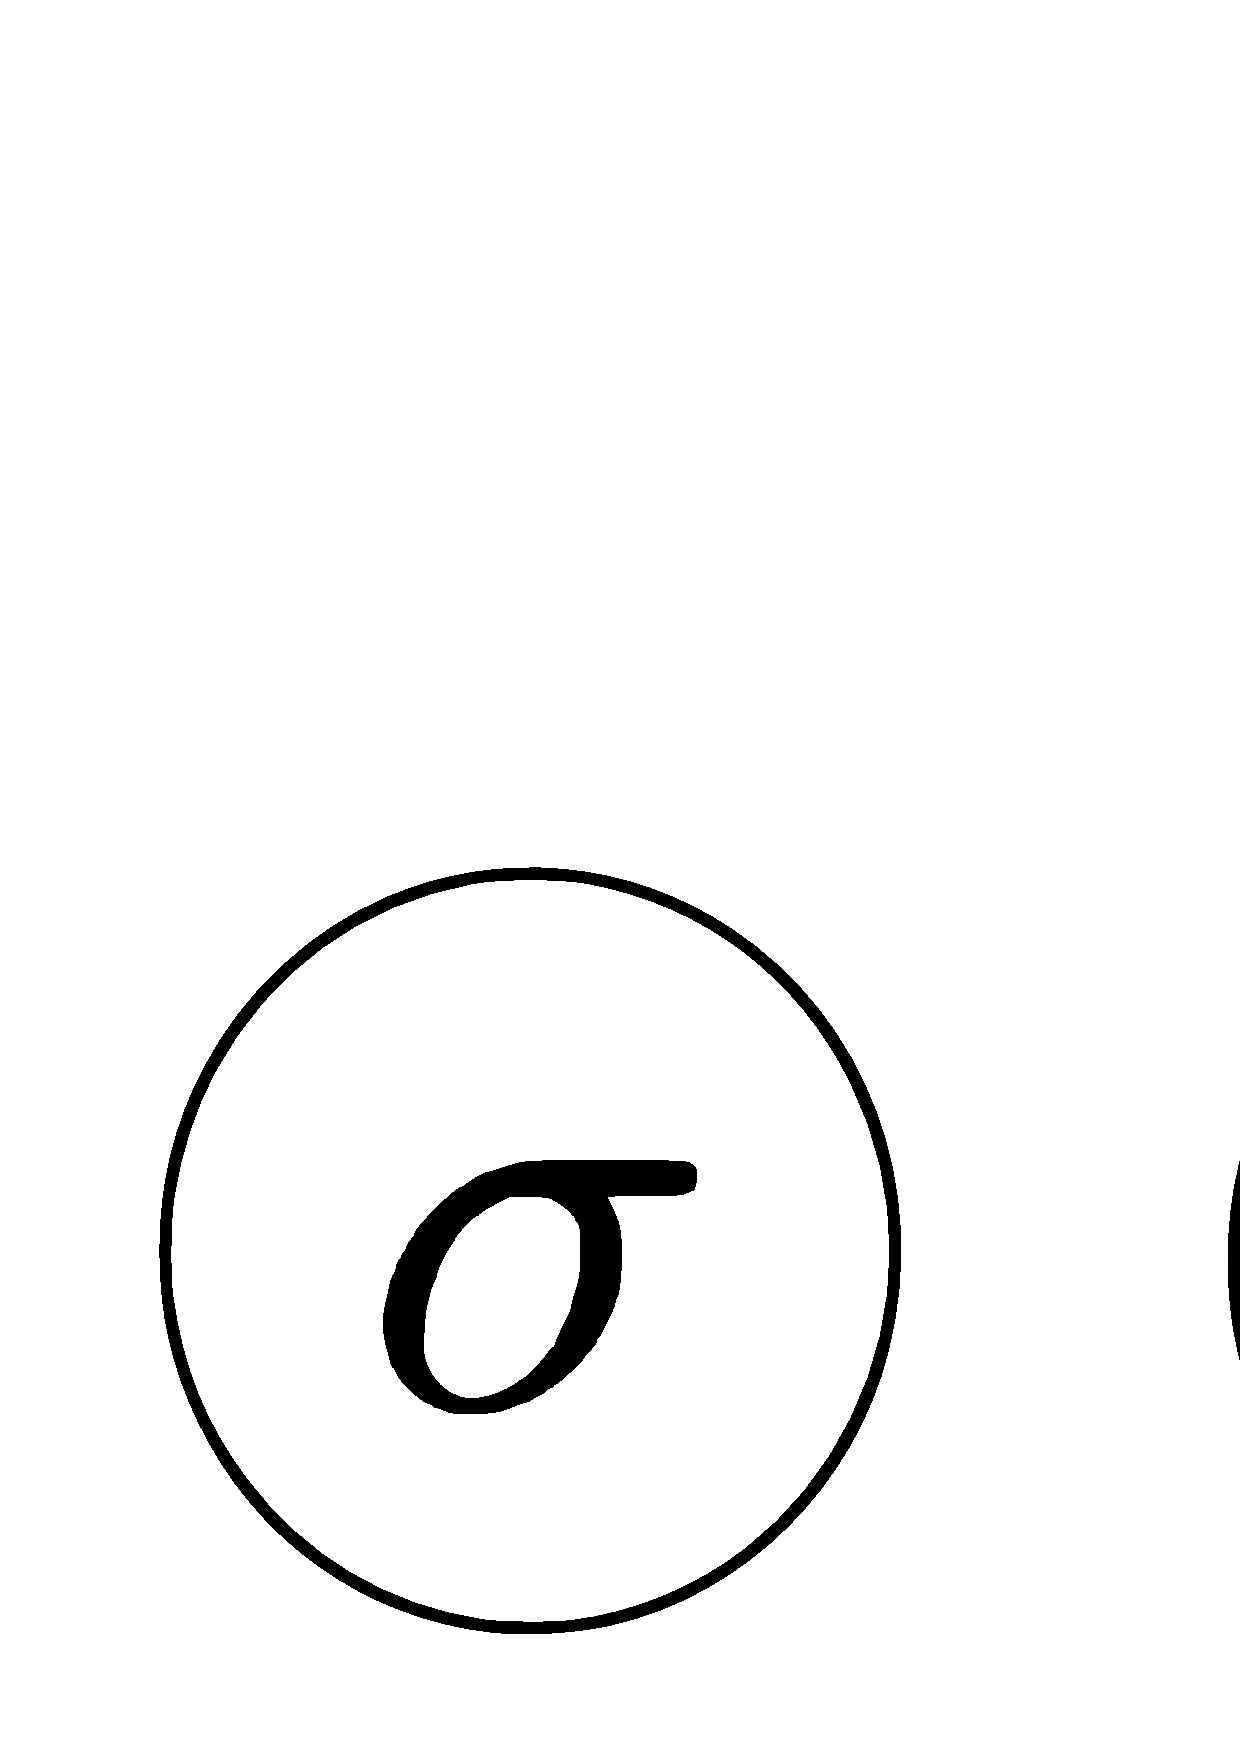
\includegraphics[width=100mm]{theorem1_src.png}
\end{figure}

\begin{figure}[!h]
	\centering
	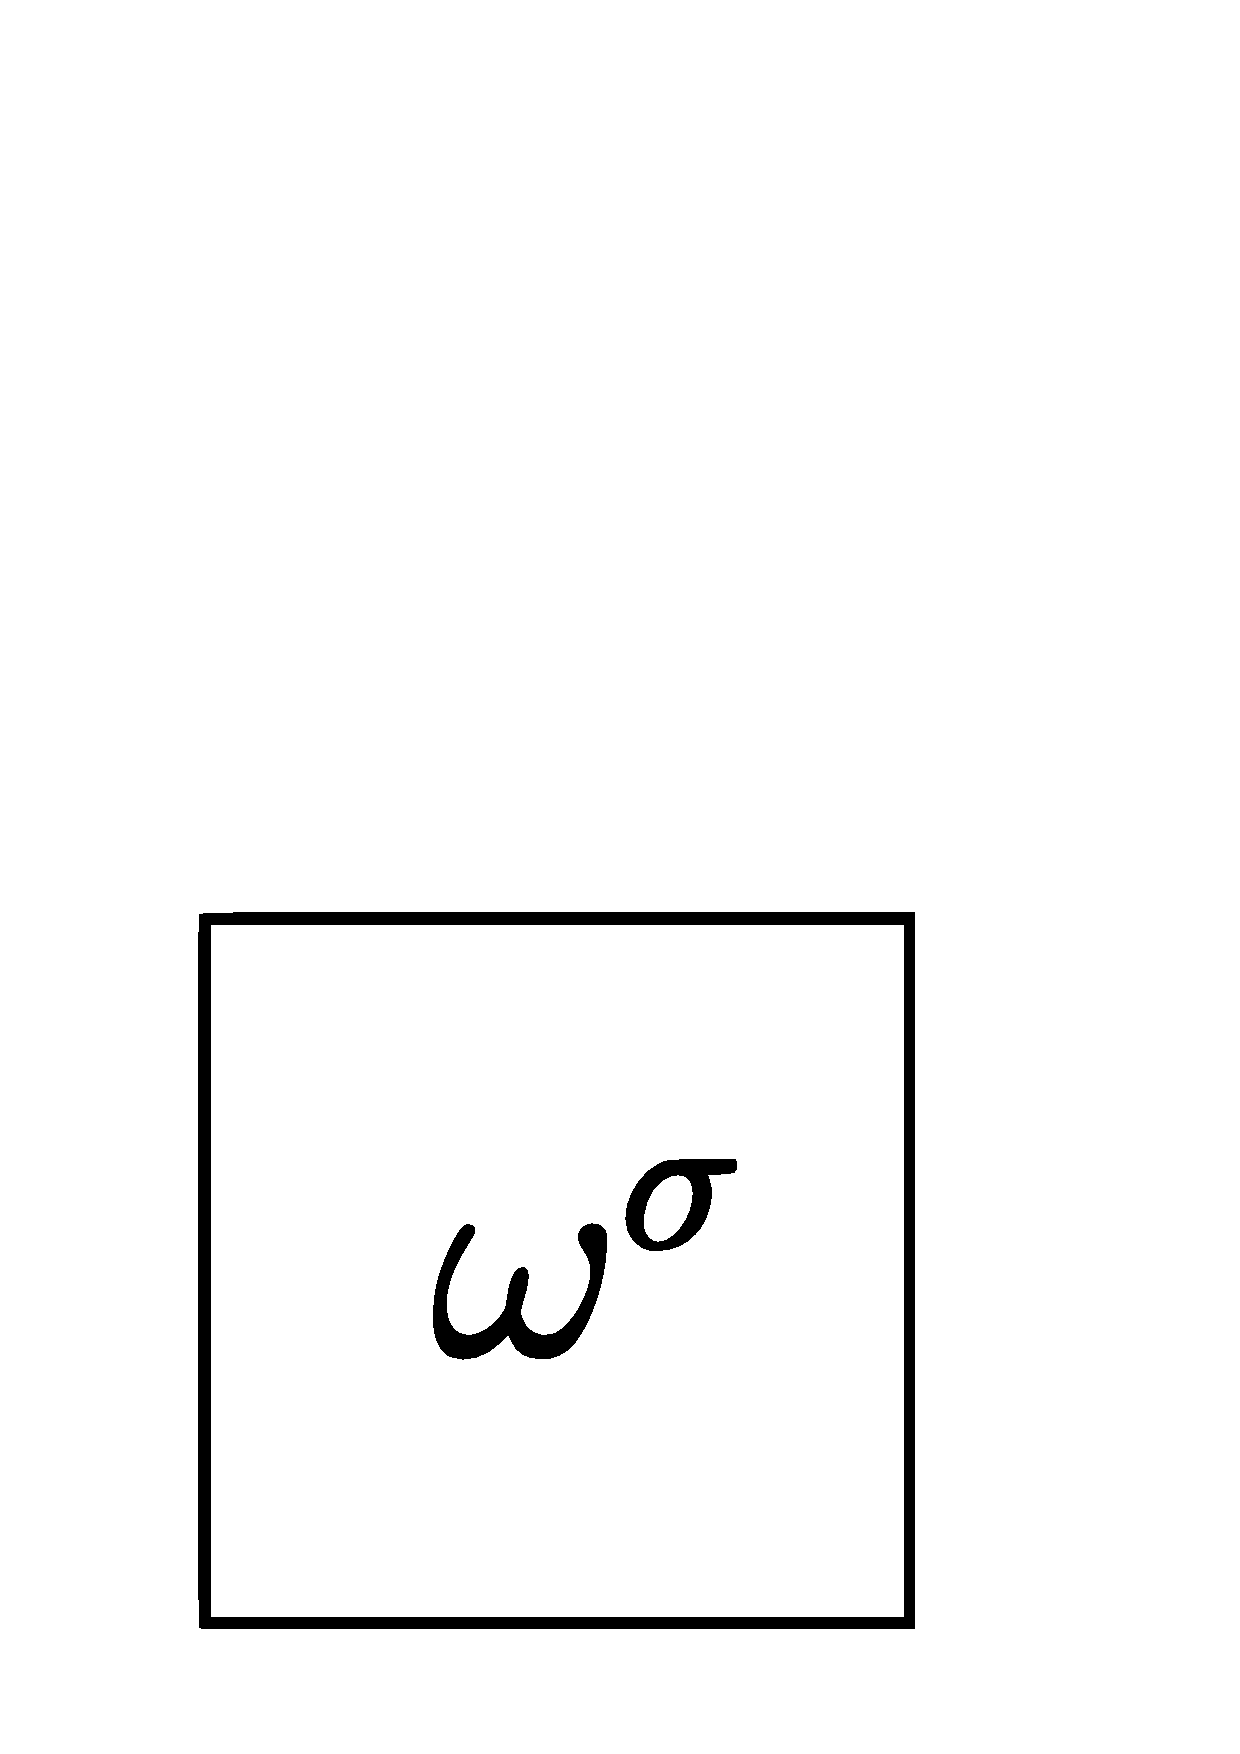
\includegraphics[width=100mm]{theorem1_dst.png}
\end{figure}
\end{frame}

\newcommand{\butpartial}{{\sigma\setminus\rho\setminus\partial_1}}
\newcommand{\butpartialA}{{\alpha\setminus{\partial_2}}}
\newcommand{\sigmanoro}{{\sigma\setminus\rho}}

\begin{frame}{Теорема об~инкрементальной компиляции}
Пусть дано: $\sigma \subset \Sigma$, $gen(\varnothing, \sigma) = \omega^\sigma$. Пусть $\rho, \alpha \subset \Sigma$, при этом $\rho \subseteq \sigma$, $\sigma \cap \alpha = \varnothing$; $\Delta = \Delta^\rho_\alpha\sigma = \sigma\setminus\rho\cup\alpha$. Известно, что определено $gen(\omega^\sigma_{\sigma\setminus\rho}, \alpha) = \omega_\alpha$ и $gen(\varnothing, \Delta) = \omega^\Delta$.
Обозначим 
$$\partial_1 = \partial\dfrac{\omega^\sigma_\rho}{\omega_\alpha}(\sigma\setminus\rho)$$
$$\omega^1_{\partial_1} = gen(\omega^\sigma_{\butpartial} \cup \omega_\alpha, \partial_1)$$
$$\partial_2 = \partial\dfrac{\omega^\sigma_{\sigma\setminus\rho}}{\omega^\sigma_{\butpartial} \cup \omega^1_{\partial_1}}(\alpha)$$
$$\omega^2_{\partial_2} = gen(\omega^\sigma_{\butpartial} \cup \omega_{\butpartialA} \cup \omega^1_{\partial_1}, \partial_2)$$
Тогда:
$$gen(\varnothing, \Delta) =^2 \omega^\sigma_{\butpartial} \cup \omega_{\butpartialA} \cup \omega^1_{\partial_1} \cup \omega^2_{\partial_2}$$

\end{frame}

\begin{frame}{Переиспользование порождений}
\begin{figure}[!h]
	\centering
	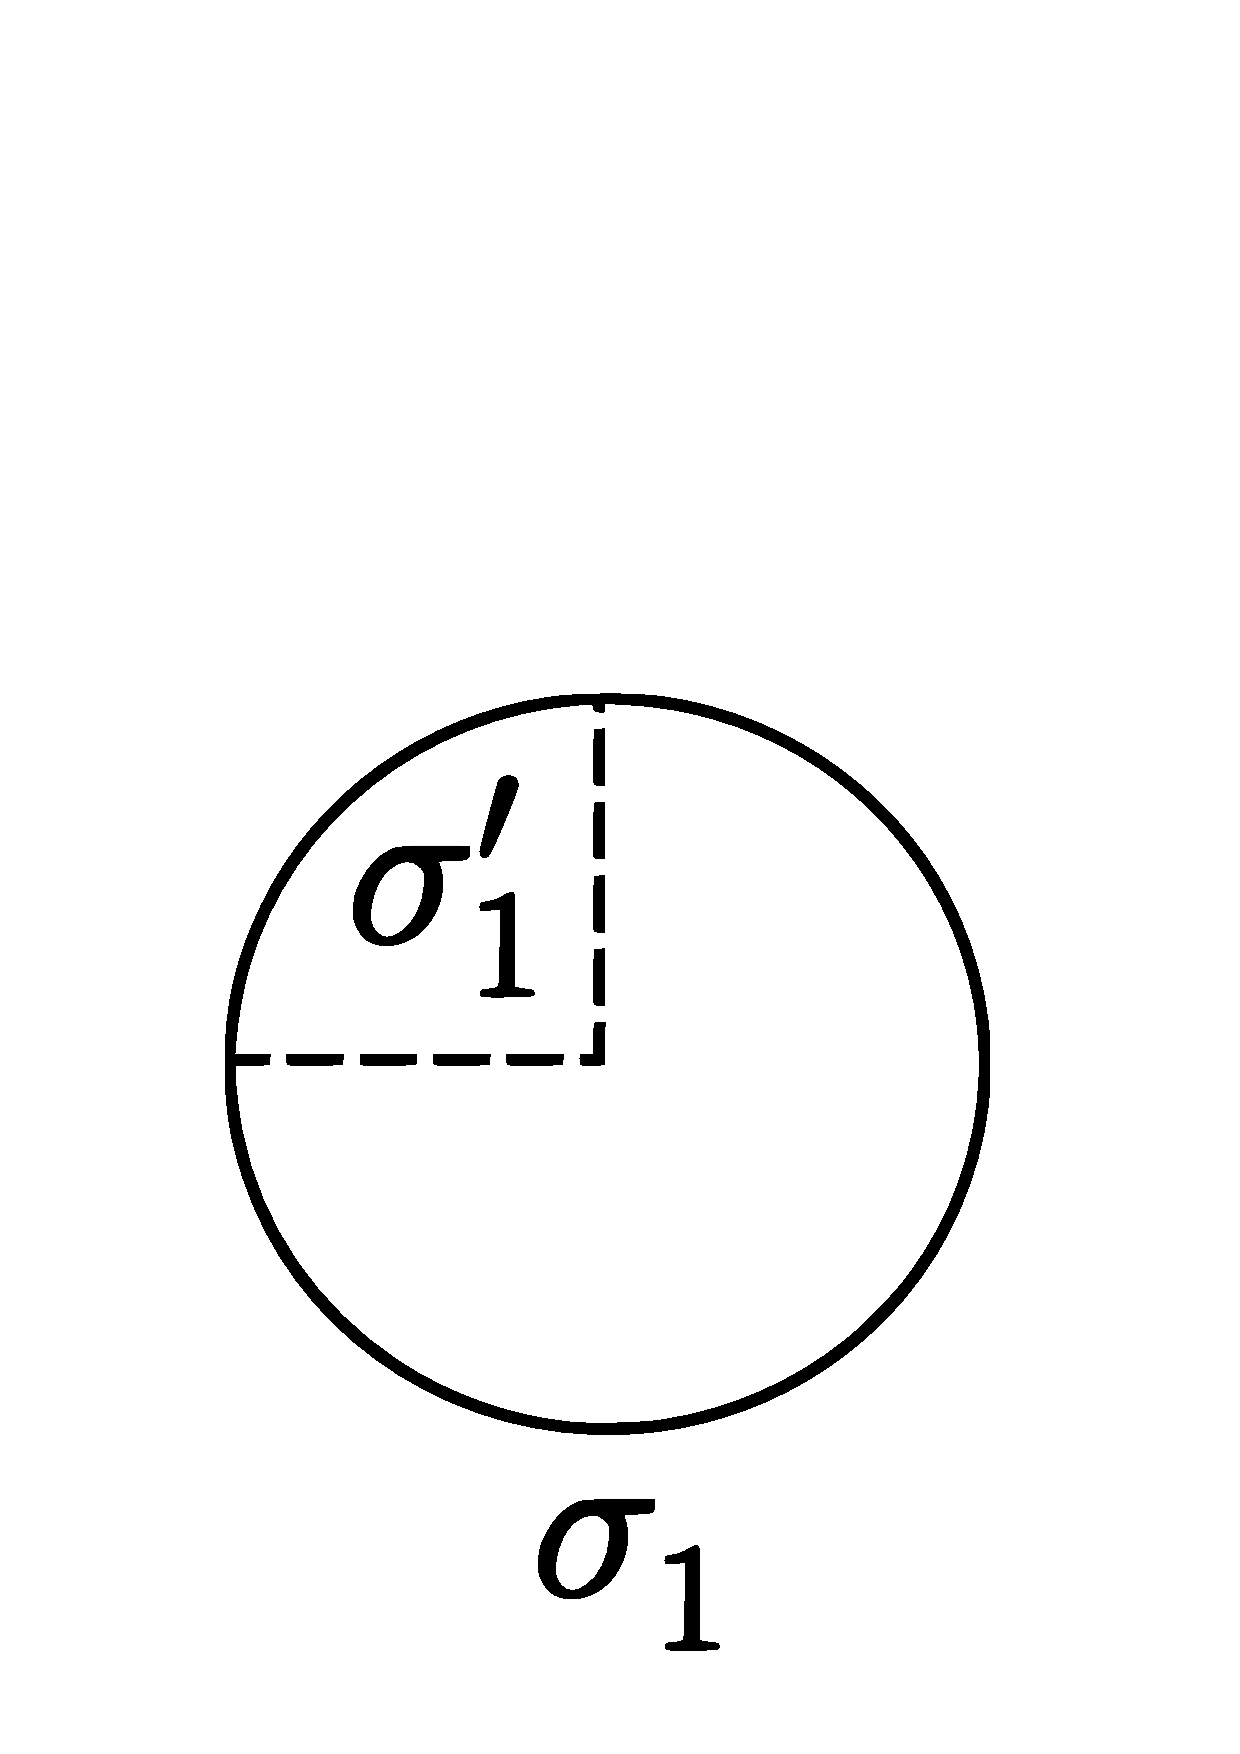
\includegraphics[width=100mm]{theorem2_src.png}
\end{figure}

\begin{figure}[!h]
	\centering
	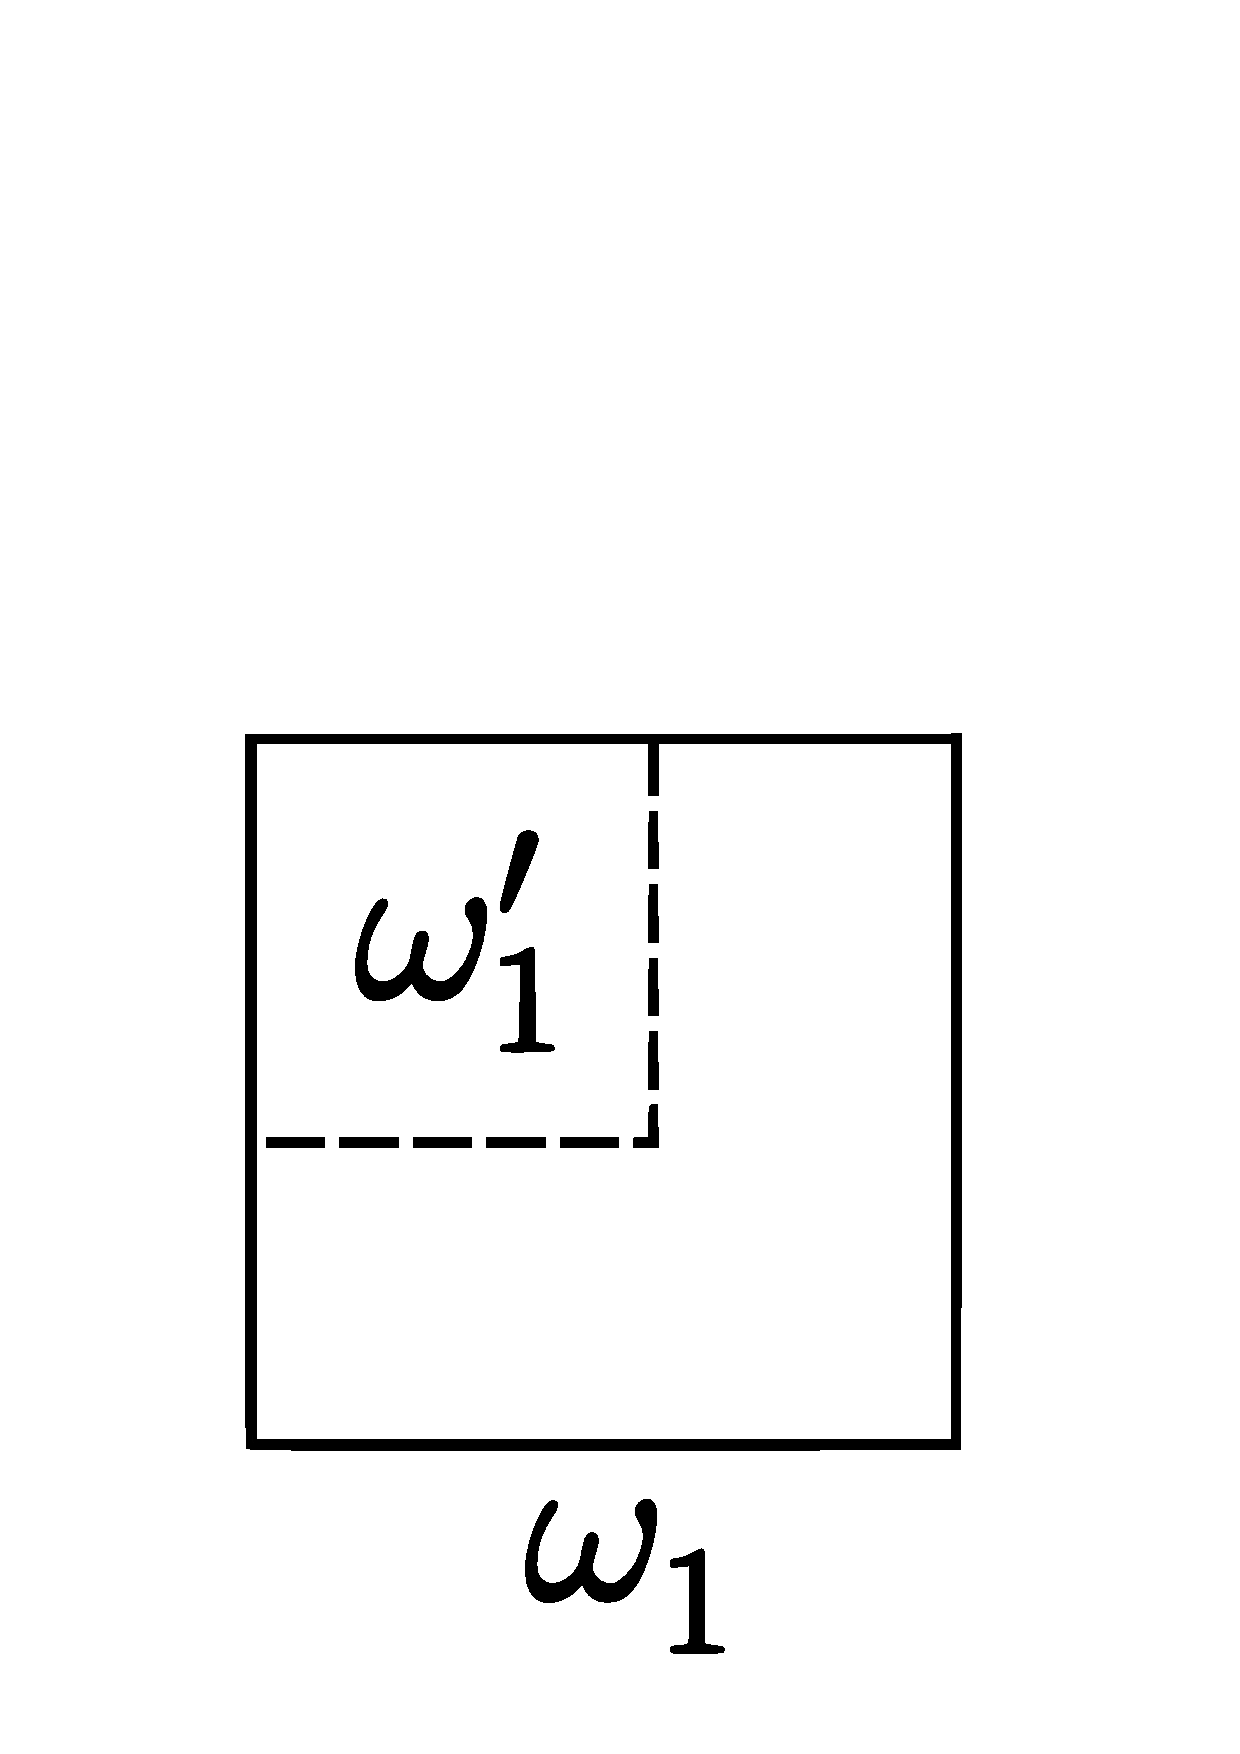
\includegraphics[width=100mm]{theorem2_dst.png}
\end{figure}
\end{frame}

\begin{frame}{Переиспользование порождений}
\begin{figure}[!h]
	\centering
	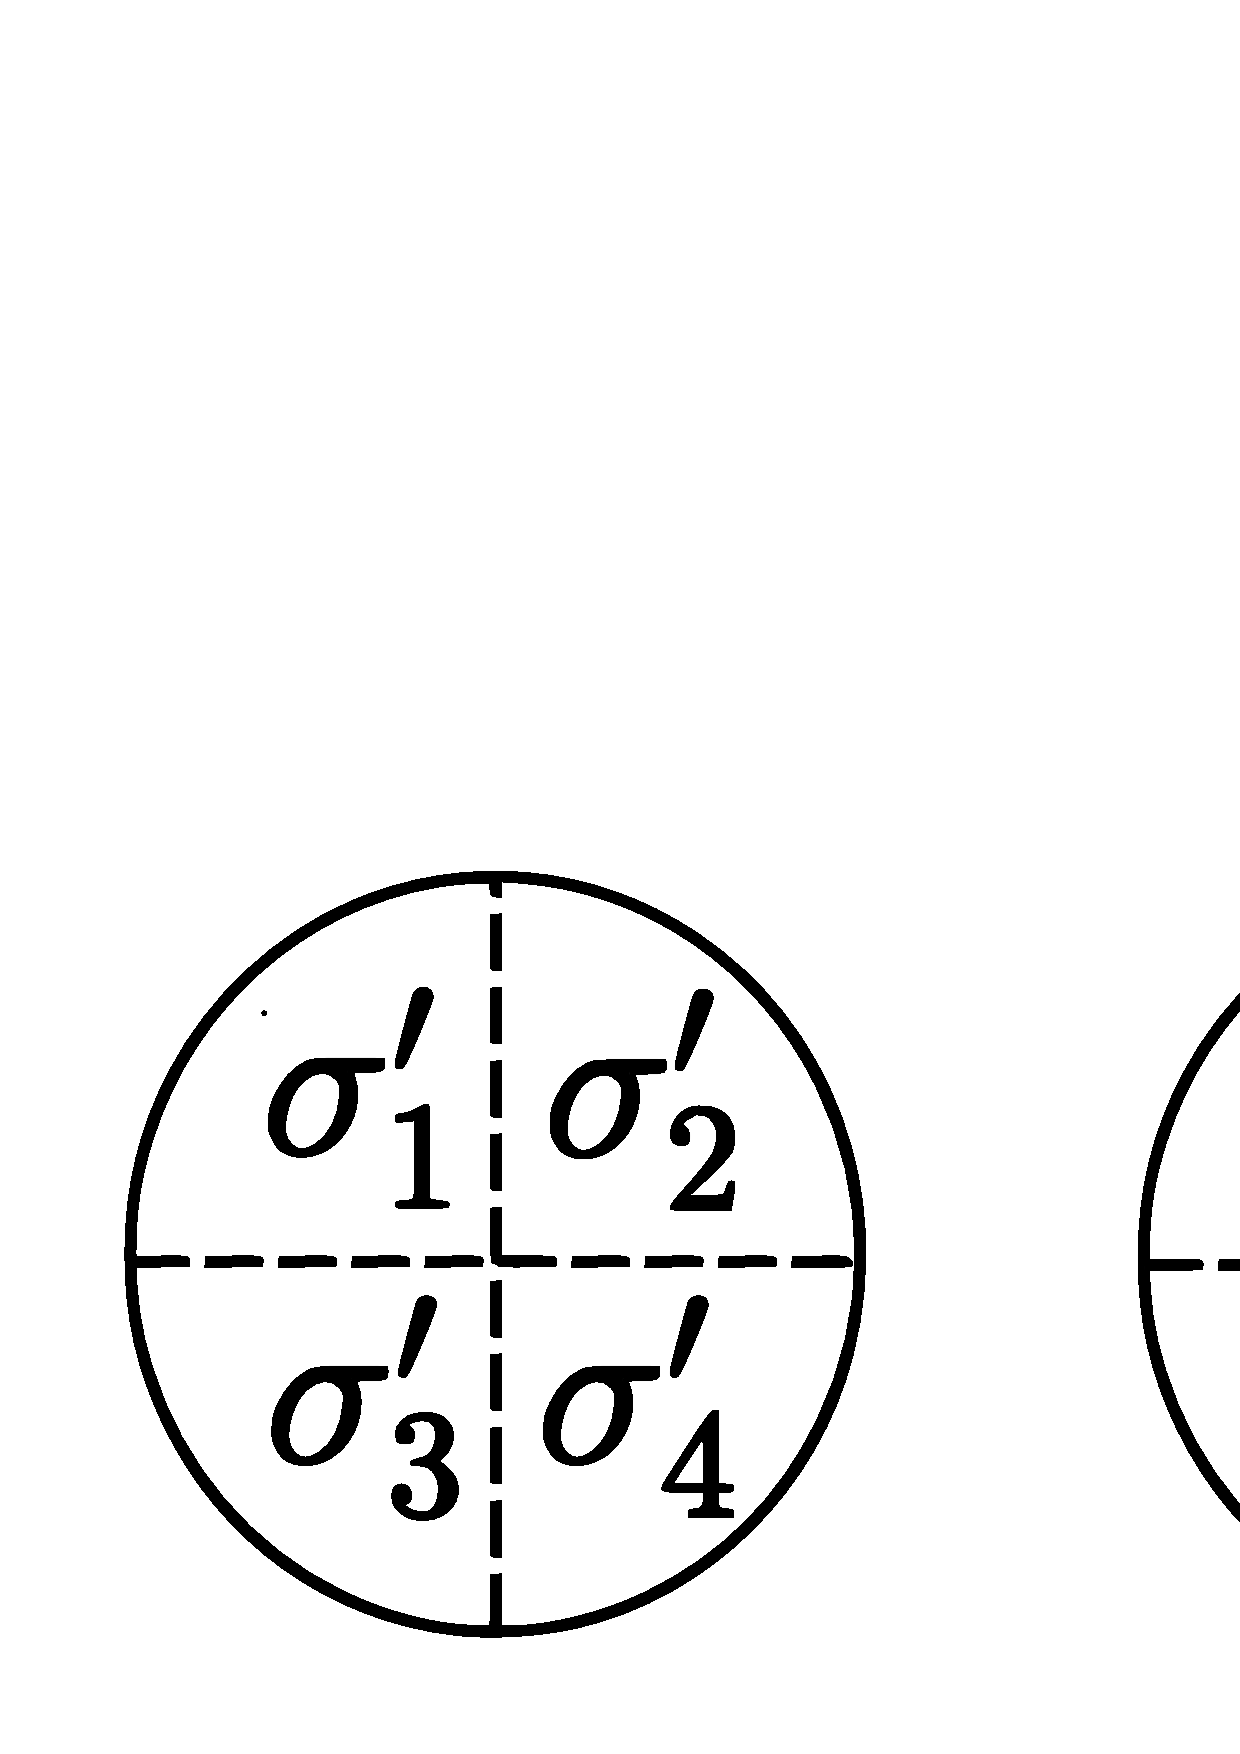
\includegraphics[width=100mm]{theorem2_srcn.png}
\end{figure}

\begin{figure}[!h]
	\centering
	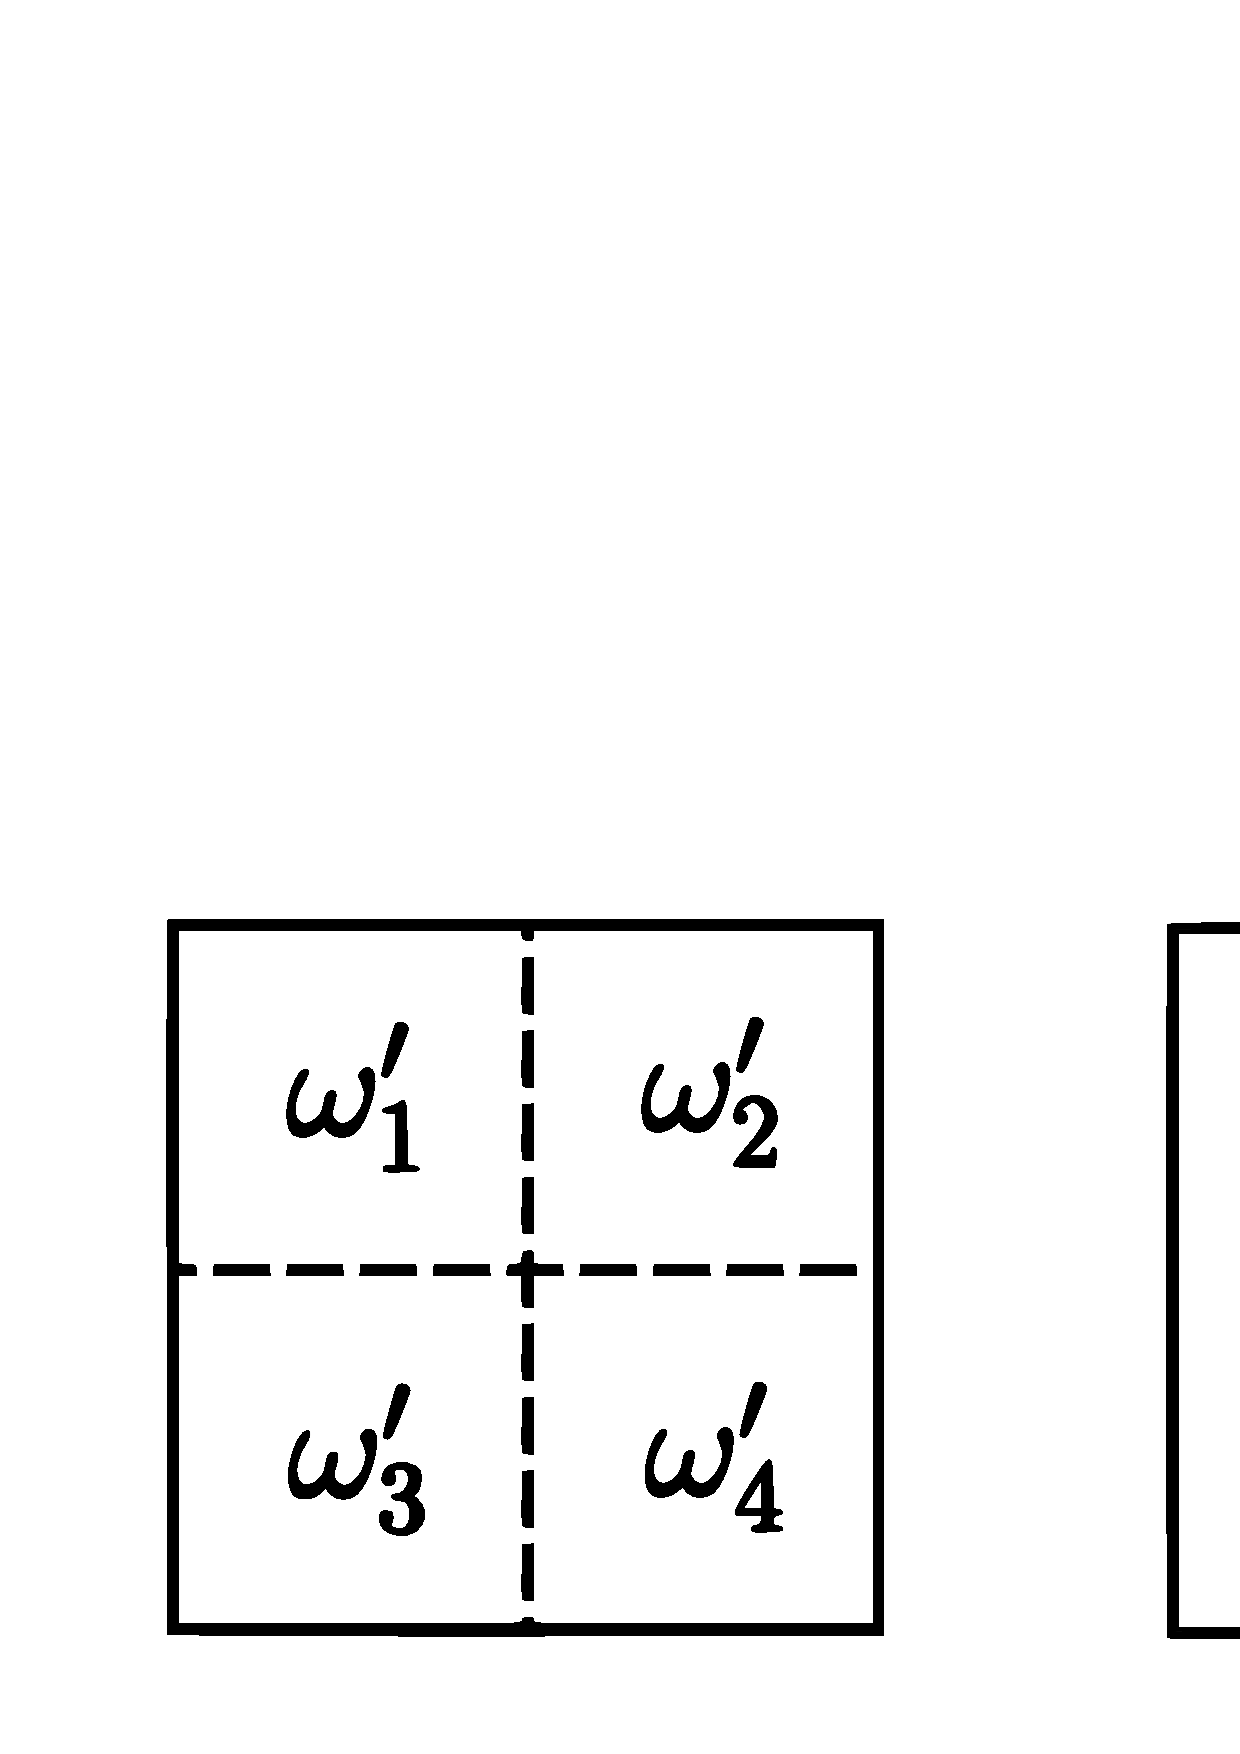
\includegraphics[width=100mm]{theorem2_dstn.png}
\end{figure}
\end{frame}

\newcommand{\sigi}{{\sigma_i}}
\newcommand{\sigk}{{\sigma_k}}
\newcommand{\sigpi}{{\sigma^\prime_i}}
\newcommand{\sigpj}{{\sigma^\prime_j}}
\newcommand{\sigpk}{{\sigma^\prime_k}}
\newcommand{\parti}{{\partial_i}}
\newcommand{\partj}{{\partial_j}}
\newcommand{\partk}{{\partial_k}}
\newcommand{\xii}{{\xi_i}}
\newcommand{\xij}{{\xi_j}}
\newcommand{\xik}{{\xi_k}}
\newcommand{\sms}{{\setminus}}
\newcommand{\alloth}{\bigcup\limits_{j \neq i}\omega^\prime_j}
\newcommand{\allothk}{\bigcup\limits_{j \neq k}\omega^\prime_j}
\newcommand{\allothD}{\bigcup\limits_{j \neq i}\omega^\Delta_{\sigpj}}
\newcommand{\rprt}{{\text{п.ч.}}}

\begin{frame}{Теорема о~переиспользовании порождений}
Пусть $\forall i \in [1:n]$ дано: $\sigma_i$, $\omega_i = gen(\varnothing, \sigma_i)$, $\sigma_i^\prime \subseteq \sigma_i$ ($\sigma_i^\prime \cap \sigma_j^\prime = \varnothing$ при $i \neq j$). Обозначим $\omega_i^\prime = gen_i(\sigma_i^\prime)$. Обозначим 
$$\partial_i = \partial\dfrac{\omega_i \setminus \omega_i^\prime}{\bigcup\limits_{j \neq i} \omega_j^\prime} (\sigma_i^\prime)$$
$$\omega_{\bigcup\limits_k \partk} = gen(\bigcup\limits_k \omega_{\sigpk\sms\partk}, \bigcup\limits_k \partk)$$
$$\xi_i = \partial\dfrac{\omega_{\sigi\sms\sigpi \cup \parti}}{\bigcup\limits_{j \neq i} \omega_{\sigpj\sms\partj} \cup \omega_{\bigcup\limits_k \partial_k}} (\sigpi\sms\parti)$$
Тогда:
$$gen(\varnothing, \bigcup\limits_k \sigpk) =^2 \bigcup\limits_k \omega_{\sigpk\sms\partk\sms\xik} \cup \omega_{\bigcup\limits_k \partial_k} \cup gen(\bigcup\limits_k \omega_{\sigpk\sms\partk\sms\xik} \cup \omega_{\bigcup\limits_k \partial_k}, \bigcup\limits_k \xik)$$

\end{frame}

\begin{frame}{Результаты}
\begin{itemize}
	\item Построена формальная модель предметной области
	\item Построена аксиоматика, отражающая свойства и~ограничения реального мира и~позволяющая доказывать нетривиальные утверждения
	\item Сформулированы и доказаны конструктивные теоремы об~инкрементальной компиляции и~переиспользовании порождений
	\item На~основе второй теоремы планируется реализовать поддержку переиспользования кэшей в~IntelliJ~IDEA
\end{itemize}
\end{frame}

\end{document}
